
\subsection{\ac{UV} \ac{AMBC} Instability During 6-\ac{DOF} Motion}
\label{chUV_AMBC.sec.fullAnalysisFailure}



This Section reports an experimental evaluation of \ac{AMBC} during
simultaneous motion in all \ac{DOF} which results in unstable parameter
adaptation.
%
%
%Two experiments reveal parameter
%adaptation instability in the presence of unmodeled thruster dynamics
%during thrust reversals. A third experiment does not have thrust
%reversals and parameter estimates remain stable. 
%
In the experiment the mass, drag, and gravitational terms were
initialized to parameters previously identified to model vehicle
performance (tabulated in Tables \ref{chUV_AMBC.tb.quasistatic} and
\ref{chUV_AMBC.tb.dynParam}). The reference trajectory specified was
RefTraj1 from Table \ref{chUV_AMBC.tb.expStat}. The gains used
were $k_p=300$, $k_d=100$ $\gamma_{m_i}=1000$, $\gamma_{d_i}=5000$,
$\gamma_{g}=\gamma_{b_1}=\gamma_{b_2}=0.5$ and $\gamma_{b_3}=10.0$.


Tables \ref{chUV_AMBC.tb.startCloseGrav} and
\ref{chUV_AMBC.tb.startCloseDyn} tabulate the initial and final
parameters identified.  Over this two-hour duration experiment most
parameter values oscillated near their previously identified values,
however $\hat{b}_3(t)$, $\hat{m}_4(t)$, and $\hat{m}_5(t)$ adapted away
from their previously identified values.  As seen in Figure
\ref{chUV_AMBC.fig.m4_m5_Full_Param_Est}, these mass estimates adapt
to physically unrealistic negative values and show no signs of
asymptotic behavior.  
%
The instability observed in this experiment motivated us to examine
the role of unmodeled thruster dynamics in the $\hat{m}_4(t)$ and
$\hat{m}_5(t)$ adaptation process.


\begin{table}[htbp]
\ssp
\caption{Gravitational Parameters Identified During Unstable Parameter Adaptation}
\begin{center}
\begin{tabular}{c|cccc}
      & $g$ & $b_1$ & $b_2$ & $b_3$   \\
      & {\it N} & {\it N m} & {\it N m} & {\it N m} \\ \hline
Init &  3.63 & 1.017 & 3.02 & 300   \\
Final&  -5.71   &  2.6      & 3.53     & 261 \\ 
\end{tabular}
\end{center}
\label{chUV_AMBC.tb.startCloseGrav}
\vspace*{-5mm}
\end{table}


\begin{table}[htbp]
\ssp
\caption{Mass and Drag Parameters Identified During Unstable Parameter Adaptation}
\begin{center}
\begin{tabular}{c|cccc}
 & $m_i(t_o)$ & $m_i(t_f)$ & $d_i(t_o)$ & $d_i(t_f)$ \\ \hline
Trans X \ac{DOF} & 583 {\it kg} & 583 {\it kg}& -1245 {\it $\frac{\text{N}~\text{s}^2}{\text{m}^2}$}& -1005 {\it $\frac{\text{N}~\text{s}^2}{\text{m}^2}$}\\
Trans Y \ac{DOF} & 873 {\it kg} & 769 {\it kg}& -1426 {\it $\frac{\text{N}~\text{s}^2}{\text{m}^2}$}& -1400 {\it $\frac{\text{N}~\text{s}^2}{\text{m}^2}$}\\
Trans Z \ac{DOF} & 1021 {\it kg} & 1031 {\it kg}& -3060 {\it $\frac{\text{N}~\text{s}^2}{\text{m}^2}$}& -3039 {\it $\frac{\text{N}~\text{s}^2}{\text{m}^2}$}\\
Angular X \ac{DOF} & 103.5 {\it kg $\text{m}^2$} & -1.348 {\it kg $\text{m}^2$} & -728.4 {\it N $\text{s}^2$}& -761.5  {\it N $\text{s}^2$}\\
Angular Y \ac{DOF} & 137.1 {\it kg $\text{m}^2$} & 42.5 {\it kg $\text{m}^2$} & -769.1  {\it N $\text{s}^2$}& -681.4  {\it N $\text{s}^2$}\\
Angular Z \ac{DOF} & 106.4 {\it kg $\text{m}^2$} & 41 {\it kg $\text{m}^2$} & -376.2  {\it N $\text{s}^2$}& -393.3  {\it N $\text{s}^2$}\\
\end{tabular}
\end{center}
\label{chUV_AMBC.tb.startCloseDyn}
\vspace*{-5mm}
\end{table}


\begin{center}
\begin{figure}[htbp]
  \begin{center}
    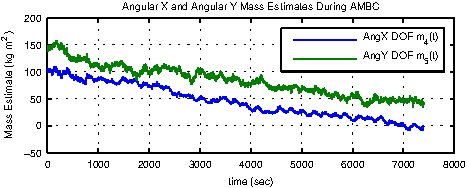
\includegraphics[width=150mm]{./chUV_AMBC/images/m4_m5_Full_Param_EstSm}
  \end{center}
  \caption{ The time evolution of Angular X \ac{DOF} and Angular Y
    \ac{DOF} mass estimates from \ac{AMBC} during 6-\ac{DOF} dynamic
    maneuvers. These mass estimates adapt to physically unrealistic
    negative values and show no signs of asymptotic behavior.}
  \label{chUV_AMBC.fig.m4_m5_Full_Param_Est}
\vspace*{-5mm}
\end{figure}
\end{center}
